\documentclass[11pt, a4paper]{article}
\usepackage{pdfpages}
\usepackage{parallel}
\usepackage[T2A]{fontenc}
%\usepackage{ucs}
\usepackage[utf8]{inputenc}
\usepackage[english,russian]{babel}
\usepackage{hyperref}
\usepackage{rotating}
\usepackage[inner=2cm,top=1.8cm,outer=2cm,bottom=2.3cm,nohead]{geometry}
%\usepackage{listings}
\usepackage{graphicx}
\usepackage{wrapfig}
\usepackage{longtable}
\usepackage{indentfirst}
\usepackage{array}
\usepackage{tikzsymbols}
\usepackage{soul}
\usepackage[ruled,vlined]{algorithm2e}
\usepackage{qrcode}
\counterwithout{figure}{section} 

\usepackage{url}
\makeatletter
\g@addto@macro{\UrlBreaks}{\UrlOrds}
\makeatother

\newcolumntype{P}[1]{>{\raggedright\arraybackslash}p{#1}}
\frenchspacing
%\usepackage{fixltx2e} %text sub- and superscripts
\usepackage{icomma} % коскі ў матэматычным рэжыме
%\PreloadUnicodePage{4}

\newcommand{\longpage}{\enlargethispage{\baselineskip}}
\newcommand{\shortpage}{\enlargethispage{-\baselineskip}}

\def\switchlang#1{\expandafter\csname switchlang#1\endcsname}
\def\switchlangbe{
\let\saverefname=\refname%
\def\refname{Літаратура}%
\def\figurename{Іл.}%
}
\def\switchlangru{
\let\saverefname=\refname%
\let\savefigurename=\figurename%
\def\refname{Литература}%
\def\figurename{Рис.}%
}
\def\switchlangen{
\let\saverefname=\refname%
\def\refname{References}%
\def\figurename{Fig.}%
}

\hyphenation{admi-ni-stra-tive}
\hyphenation{ex-pe-ri-ence}
\hyphenation{fle-xi-bi-li-ty}
\hyphenation{Py-thon}
\hyphenation{ma-the-ma-ti-cal}
\hyphenation{re-ported}
\hyphenation{imp-le-menta-tions}
\hyphenation{pro-vides}
\hyphenation{en-gi-neering}
\hyphenation{com-pa-ti-bi-li-ty}
\hyphenation{im-pos-sible}
\hyphenation{desk-top}
\hyphenation{elec-tro-nic}
\hyphenation{com-pa-ny}
\hyphenation{de-ve-lop-ment}
\hyphenation{de-ve-loping}
\hyphenation{de-ve-lop}
\hyphenation{da-ta-ba-se}
\hyphenation{plat-forms}
\hyphenation{or-ga-ni-za-tion}
\hyphenation{pro-gramming}
\hyphenation{in-stru-ments}
\hyphenation{Li-nux}
\hyphenation{sour-ce}
\hyphenation{en-vi-ron-ment}
\hyphenation{Te-le-pathy}
\hyphenation{Li-nux-ov-ka}
\hyphenation{Open-BSD}
\hyphenation{Free-BSD}
\hyphenation{men-ti-on-ed}
\hyphenation{app-li-ca-tion}

\def\progref!#1!{\texttt{#1}}
\renewcommand{\arraystretch}{2} %Іначай формулы ў матрыцы зліпаюцца з лініямі
\usepackage{array}

\def\interview #1 (#2), #3, #4, #5\par{

\section[#1, #3, #4]{#1 -- #3, #4}
\def\qname{LVEE}
\def\aname{#1}
\def\q ##1\par{{\noindent \bf \qname: ##1 }\par}
\def\a{{\noindent \bf \aname: } \def\qname{L}\def\aname{#2}}
}

\def\interview* #1 (#2), #3, #4, #5\par{

\section*{#1\\{\small\rm #3, #4. #5}}
\ifx\ParallelWhichBox\undefined%
    \addcontentsline{toc}{section}{#1, #3, #4}%
\else%
\ifnum\ParallelWhichBox=0%
    \addcontentsline{toc}{section}{#1, #3, #4}%
\fi\fi%

\def\qname{LVEE}
\def\aname{#1}
\def\q ##1\par{{\noindent \bf \qname: ##1 }\par}
\def\a{{\noindent \bf \aname: } \def\qname{L}\def\aname{#2}}
}

\newcommand{\interviewfooter}[1]{
\vskip 1em
\noindent \textit{#1}
}

\AtEndDocument{\vfill\centering \qrcode{https://github.com/fiowro/mouses/blob/main/\jobname.pdf}}

\switchlang{en}
\begin{document}

\title{1985 -- Logitech C7 mouse}
\date{}
\maketitle
\selectlanguage{english}
Logitech C7 mouse was released in 1985. It was the first mouse sold under the Logitech brand \cite{timeline}, and also its first mouse produced for retail (before that, company was focused on producing mice for OEM supplies) \cite{history}.
The selling price of the C7 was only \$100, which was noticeably cheaper than other optomechanical mice of the time. Apparently this, along with a successful construction, made the mouse very popular among end users, despite its noticeable “squareness” (fig. \ref{fig:LogitechC7Pic}).

\begin{figure}[h]
   \centering
    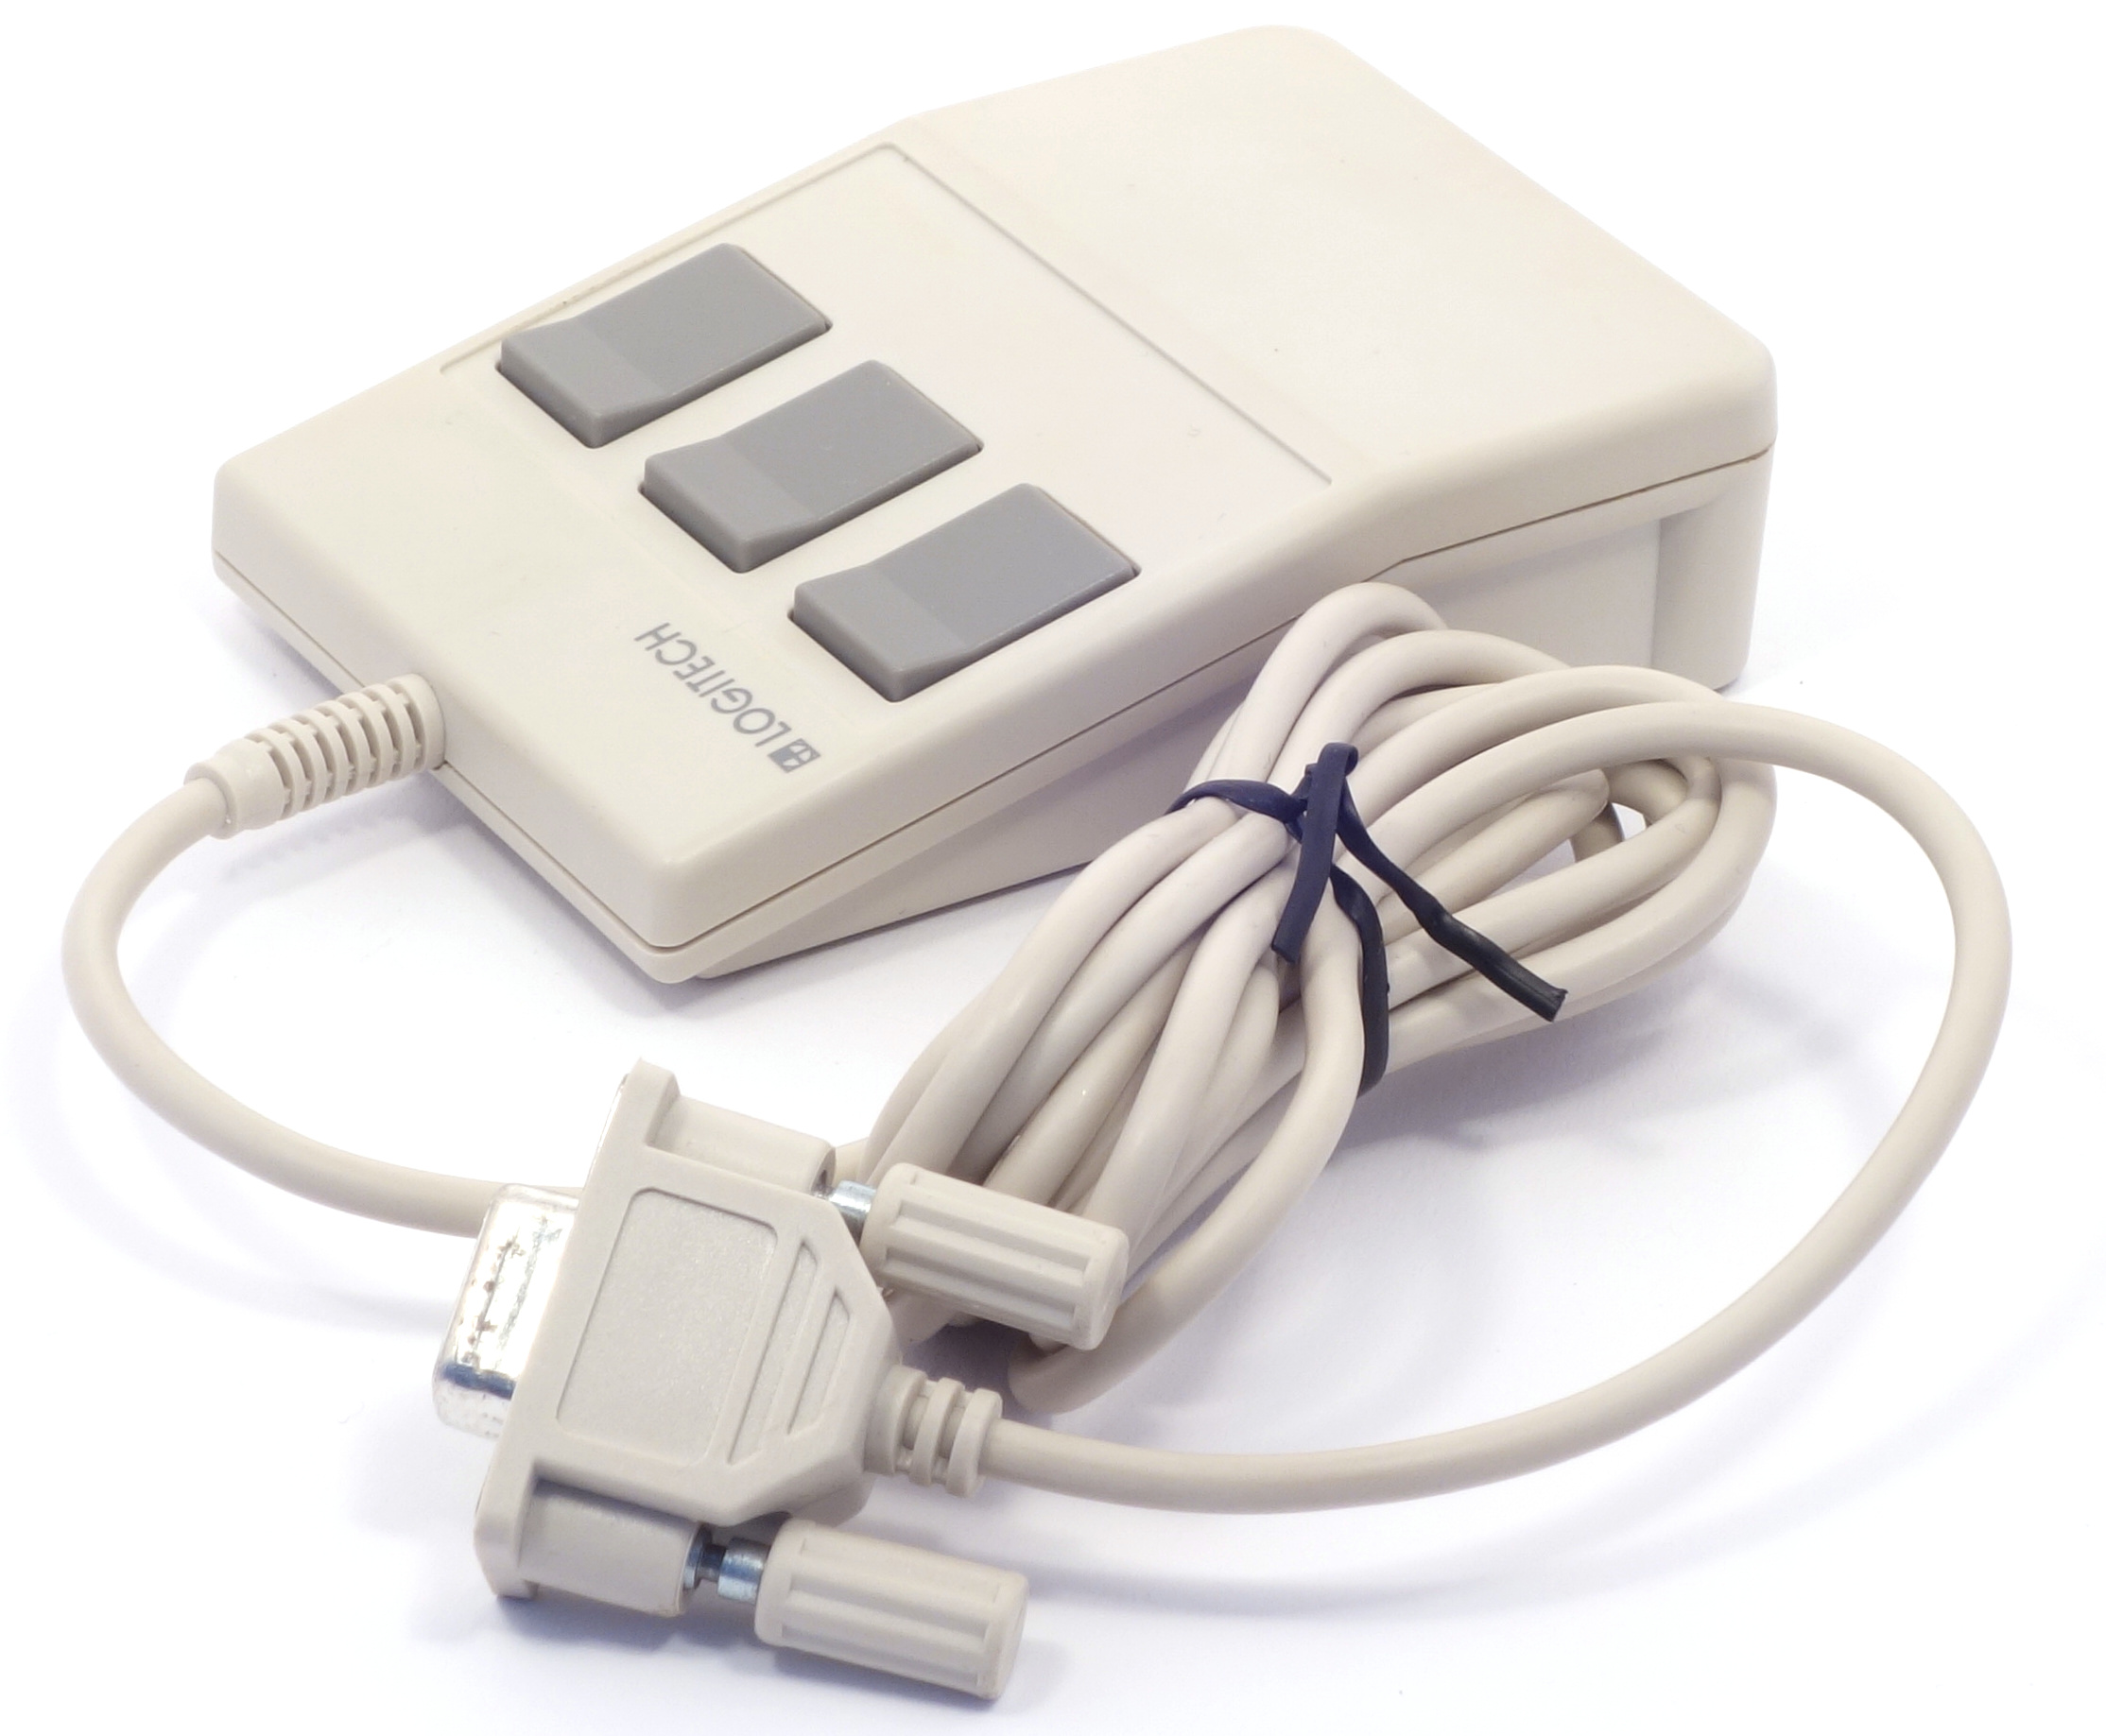
\includegraphics[scale=0.5]{1985_logitech_c7_mouse/pic_60.jpg}
    \caption{Logitech C7 mouse}
    \label{fig:LogitechC7Pic}
\end{figure}

The shape of the mouse body shows a clear resemblance to the earlier model, LOGIMOUSE P5, created with the participation of famous Swiss designer Antoine Cahen. The C7 abandoned the rigid prismatic shape of the case, providing the user with a horizontal platform for palm support, as well as slightly rounded edges and corners. Instead of the narrow diagonal buttons of the P5, the mouse received much more convenient rectangular keys with a large area (fig. \ref{fig:LogitechC7TopAndBottom}). The underside remains even more similar to the P5, also featuring four white low-friction supports (this time glued to the side of the case, which will soon become commonplace) and a removable turnable ring with latches that allows you to remove the ball and clean the rollers.

\begin{figure}[h]
    \centering
    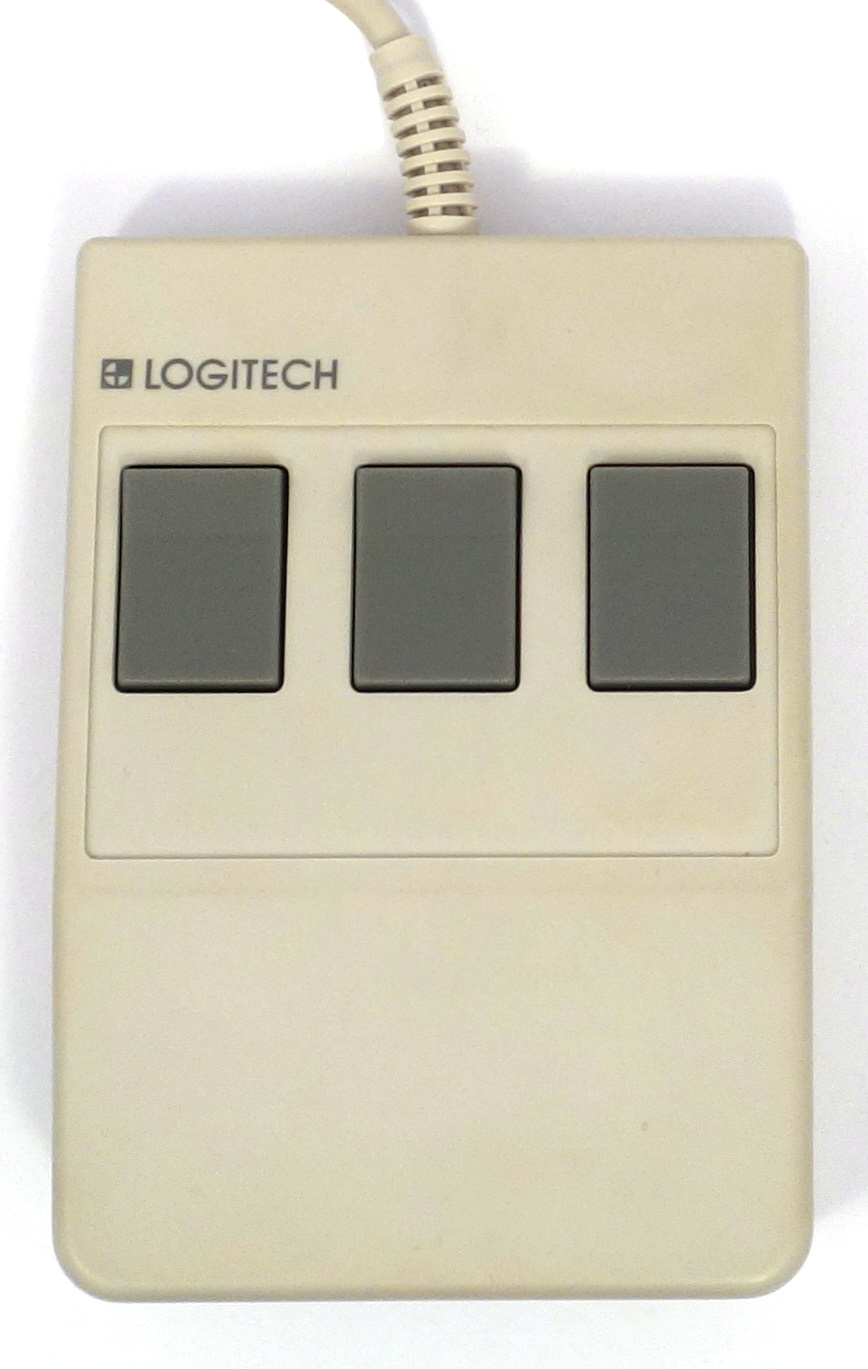
\includegraphics[scale=0.45]{1985_logitech_c7_mouse/top_30.jpg}
    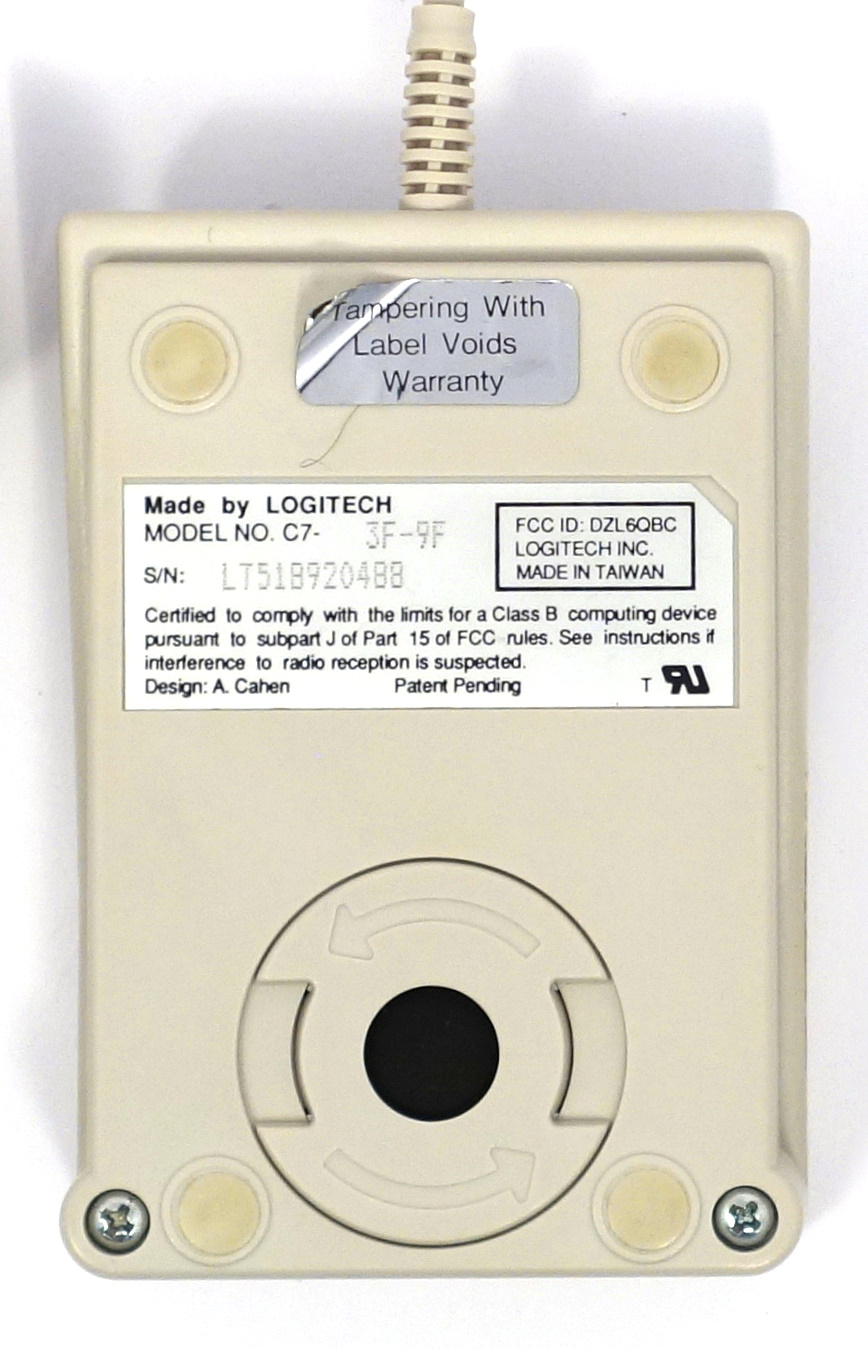
\includegraphics[scale=0.45]{1985_logitech_c7_mouse/bottom_30.jpg}
    \caption{Logitech C7 mouse, top and bottom views}
    \label{fig:LogitechC7TopAndBottom}
\end{figure}

\begin{figure}[h]
    \centering
    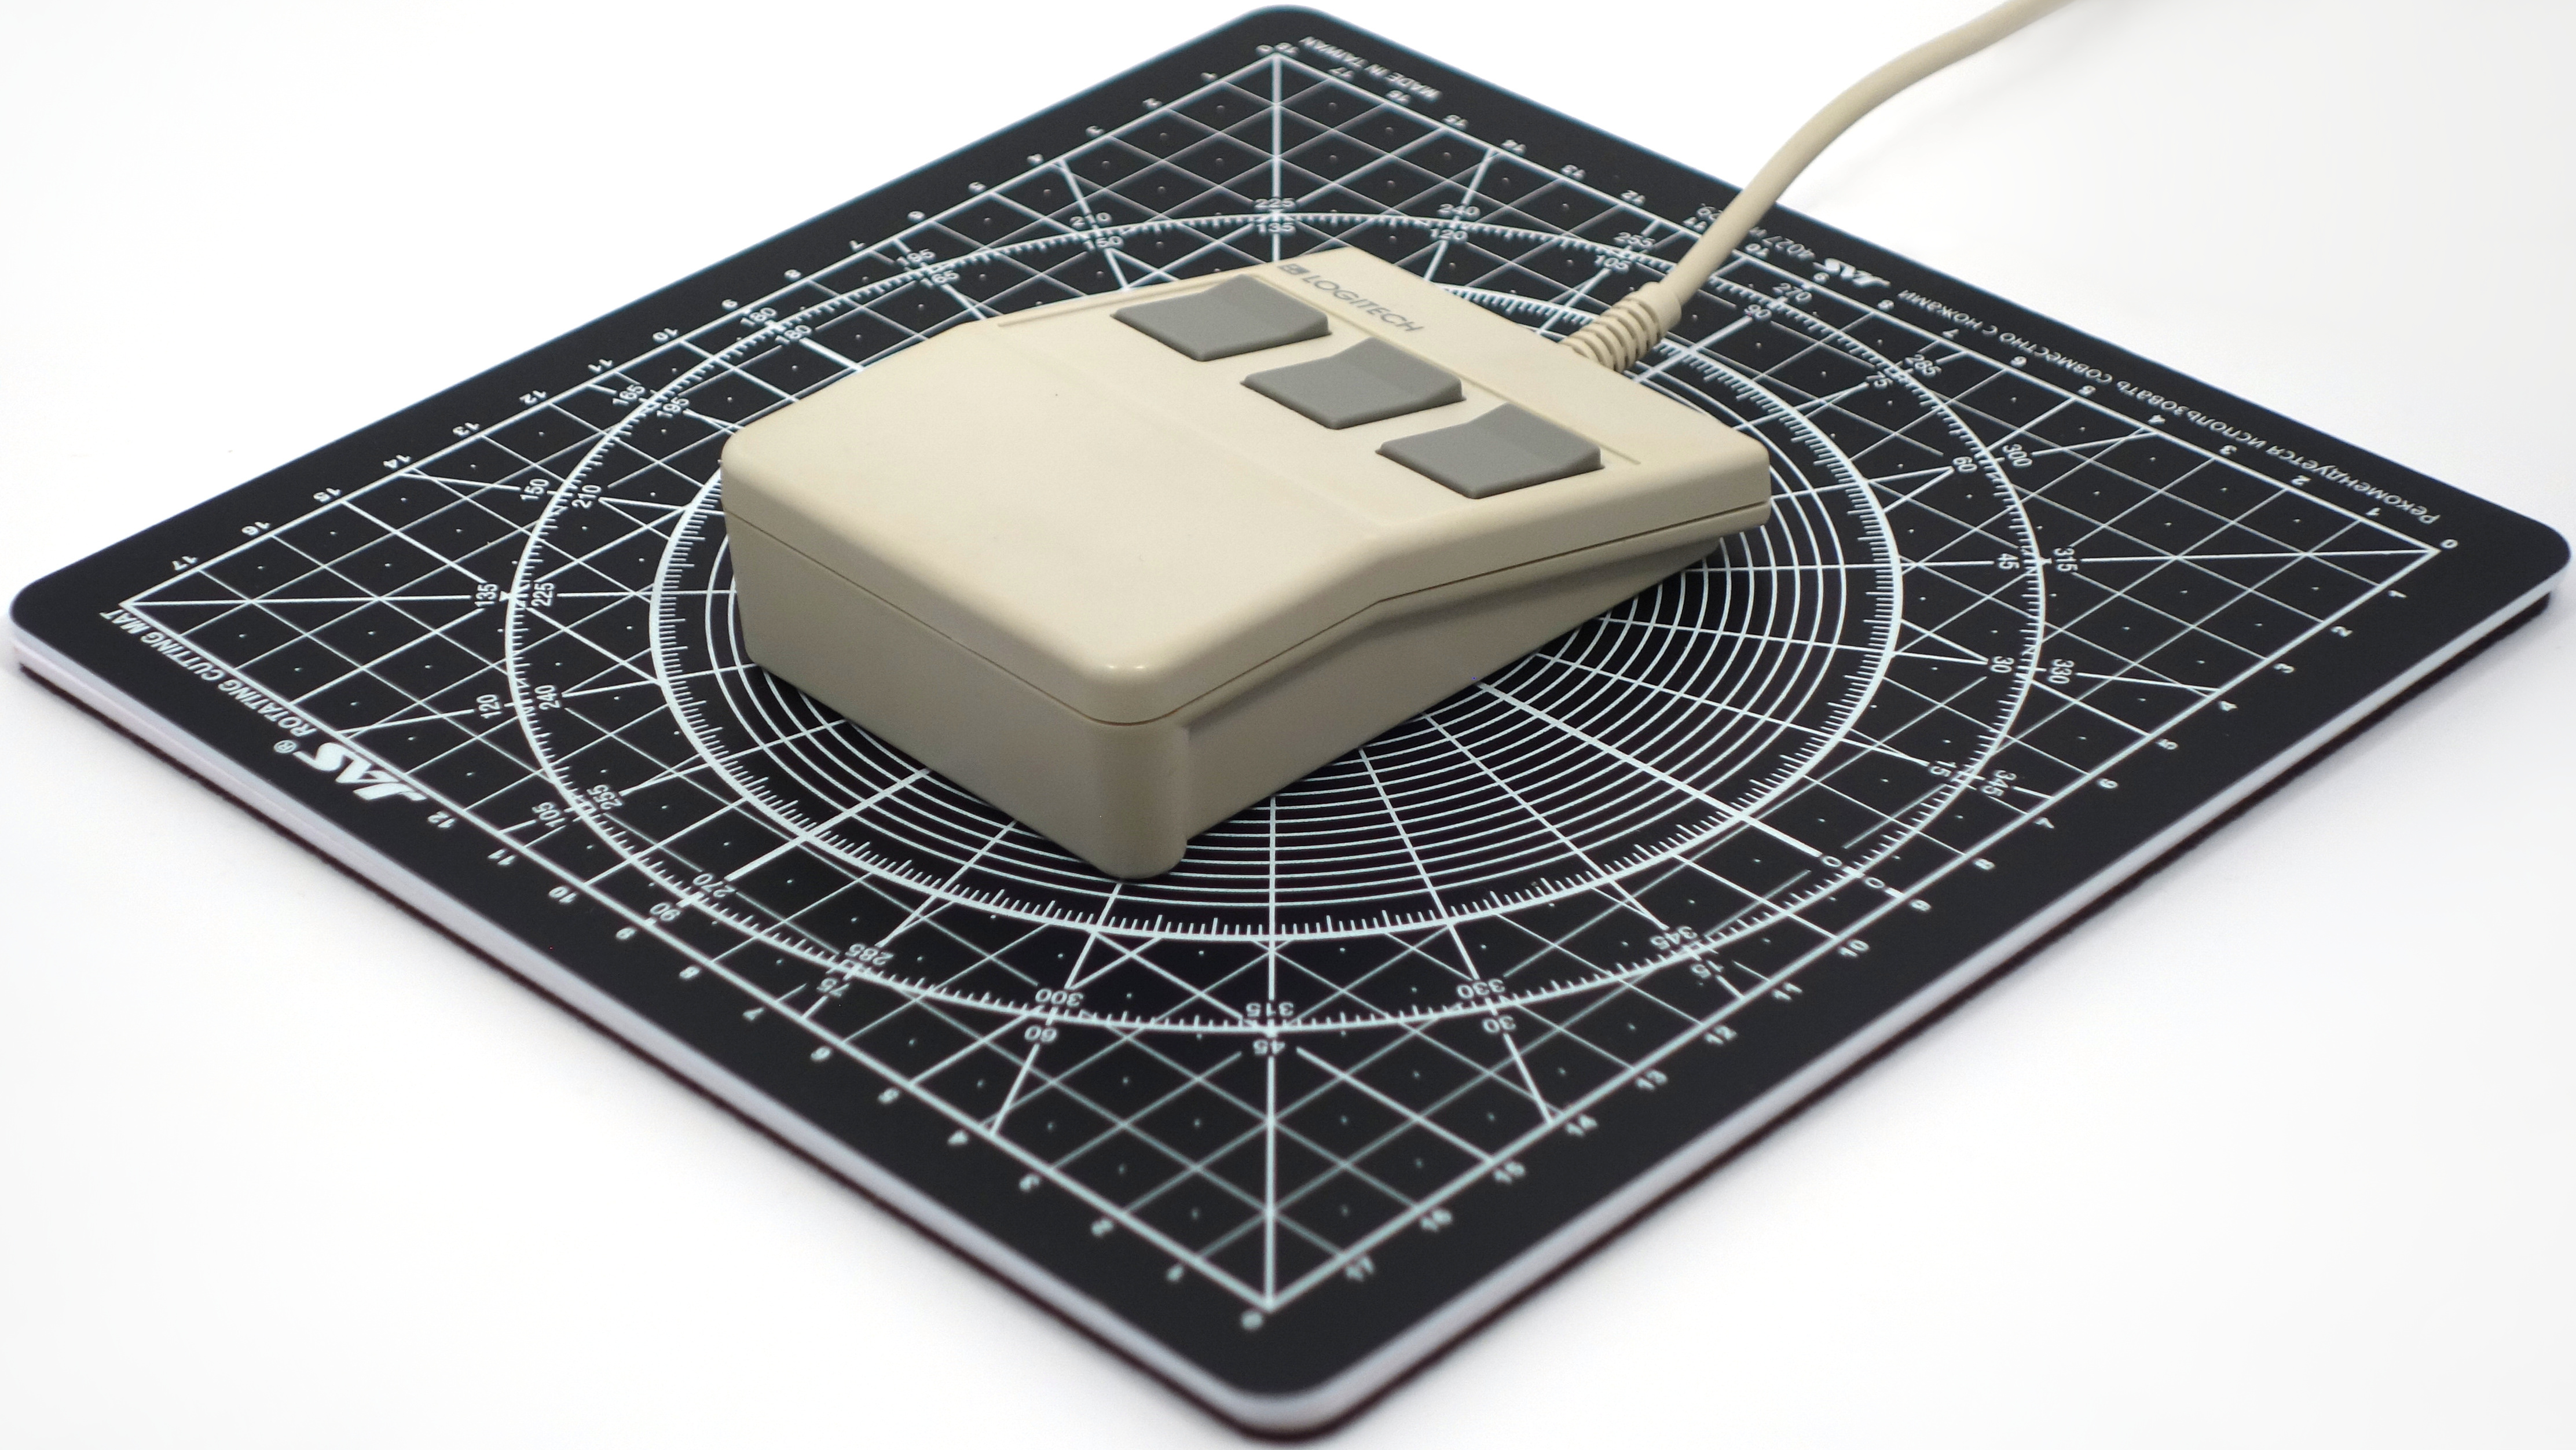
\includegraphics[scale=0.35]{1985_logitech_c7_mouse/size_30.jpg}
    \caption{Logitech C7 mouse on a graduated pad with a grid step of 1~cm}
    \label{fig:LogitechC7Size}
\end{figure}

The size of the mouse is typical for mice from the 1980s (fig. \ref{fig:LogitechC7Size}), not too different from the previous model, P5. As for ergonomics, it is obvious that a partial departure from the original design of Antoine Cahen in favor of a more pragmatic solution has benefited it. The upper body provides palm support and the buttons are comfortable enough for the fingers (fig. \ref{fig:LogitechC7Hand}) \cite{manual1, manual2}. In the early 90s, the angularity of the C7 would have looked like a disadvantage compared to mice with more curved shapes, but for the mid-80s the mouse has a good level of ergonomics.

\begin{figure}[h]
    \centering
    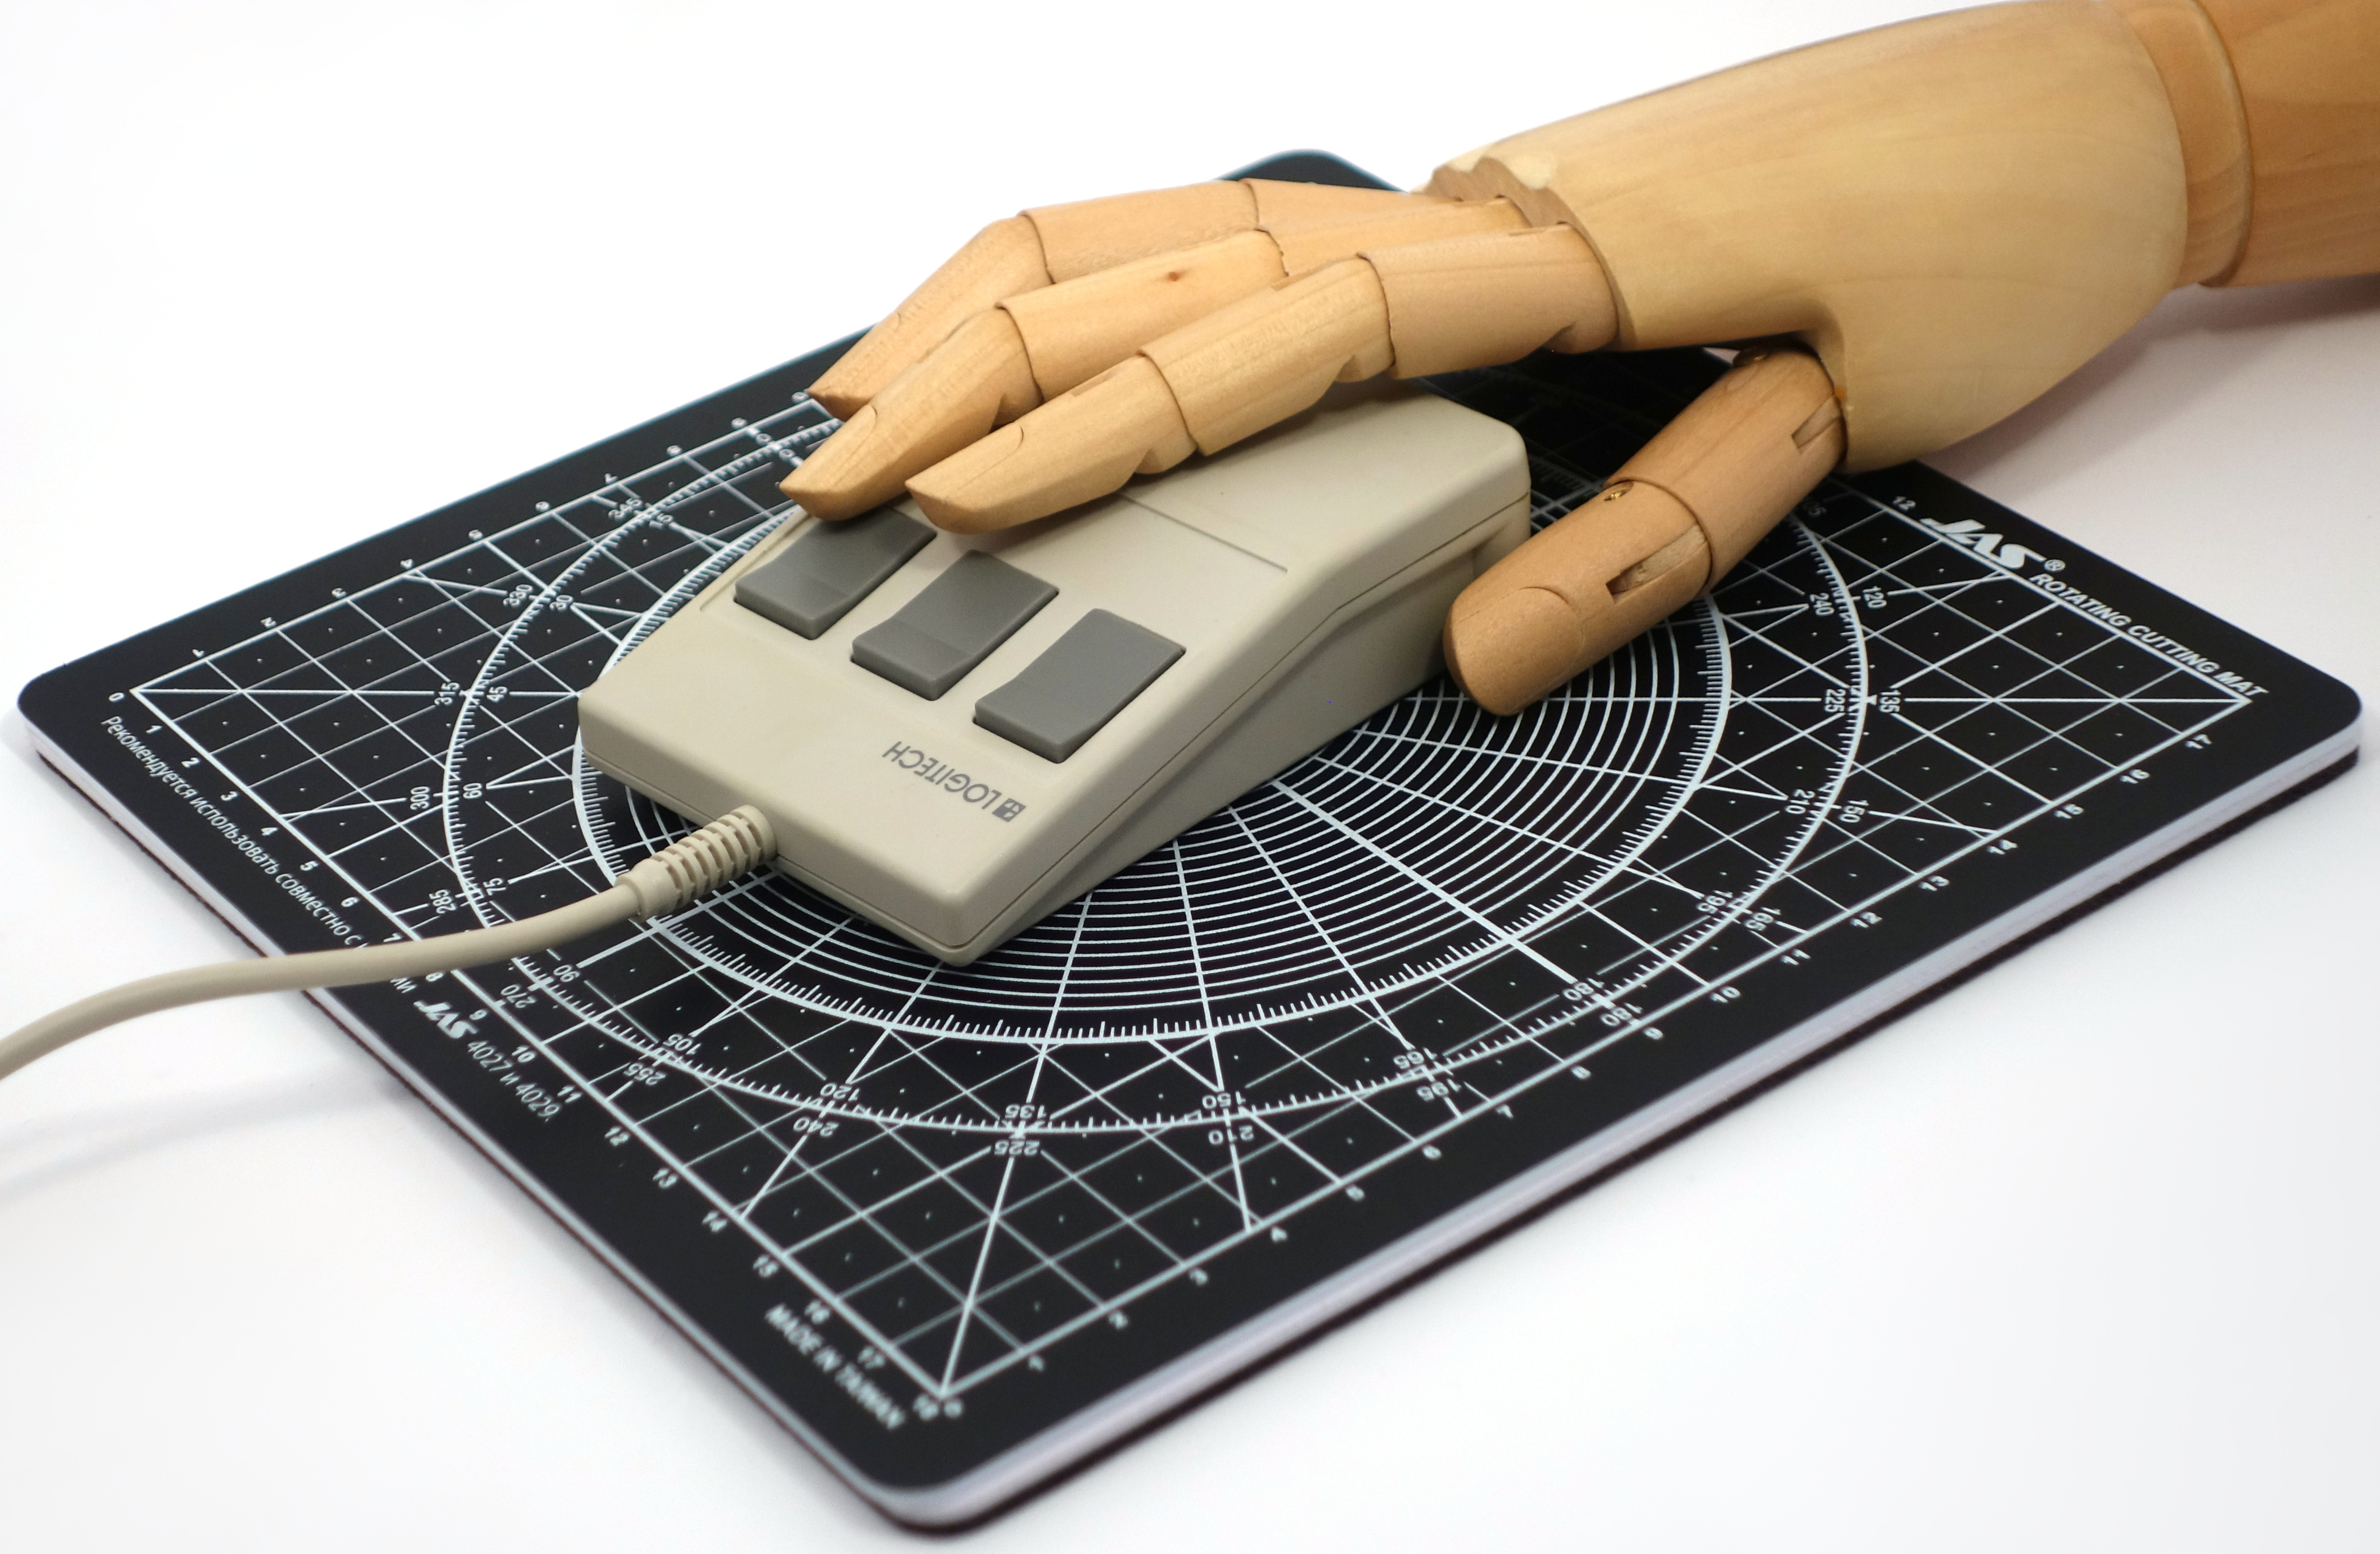
\includegraphics[scale=0.35]{1985_logitech_c7_mouse/hand_30.jpg}
    \caption{Logitech C7 mouse with a human hand model}
    \label{fig:LogitechC7Hand}
\end{figure}

The internal structure of the mouse is shown in fig. \ref{fig:LogitechC7Inside}. Like the LOGIMOUSE P5, this mouse is optomechanical. It also has a largely identical component layout to the P5, including optocouplers with an optical interrupter and the entire mechanical assembly. The differences are in a more complicated circuit design (due to the use of a serial interface), mechanical protection of the cable where it exits the body, as well as metal strips that spring the buttons. It should also be noted that the C7 was probably one of the first mice with an RS-232 interface, which used low-power LEDs and therefore did not require external power (in the case of the P5, such an issue was not relevant, since the quadrature interface provided enough power anyway).

\begin{figure}[h]
    \centering
    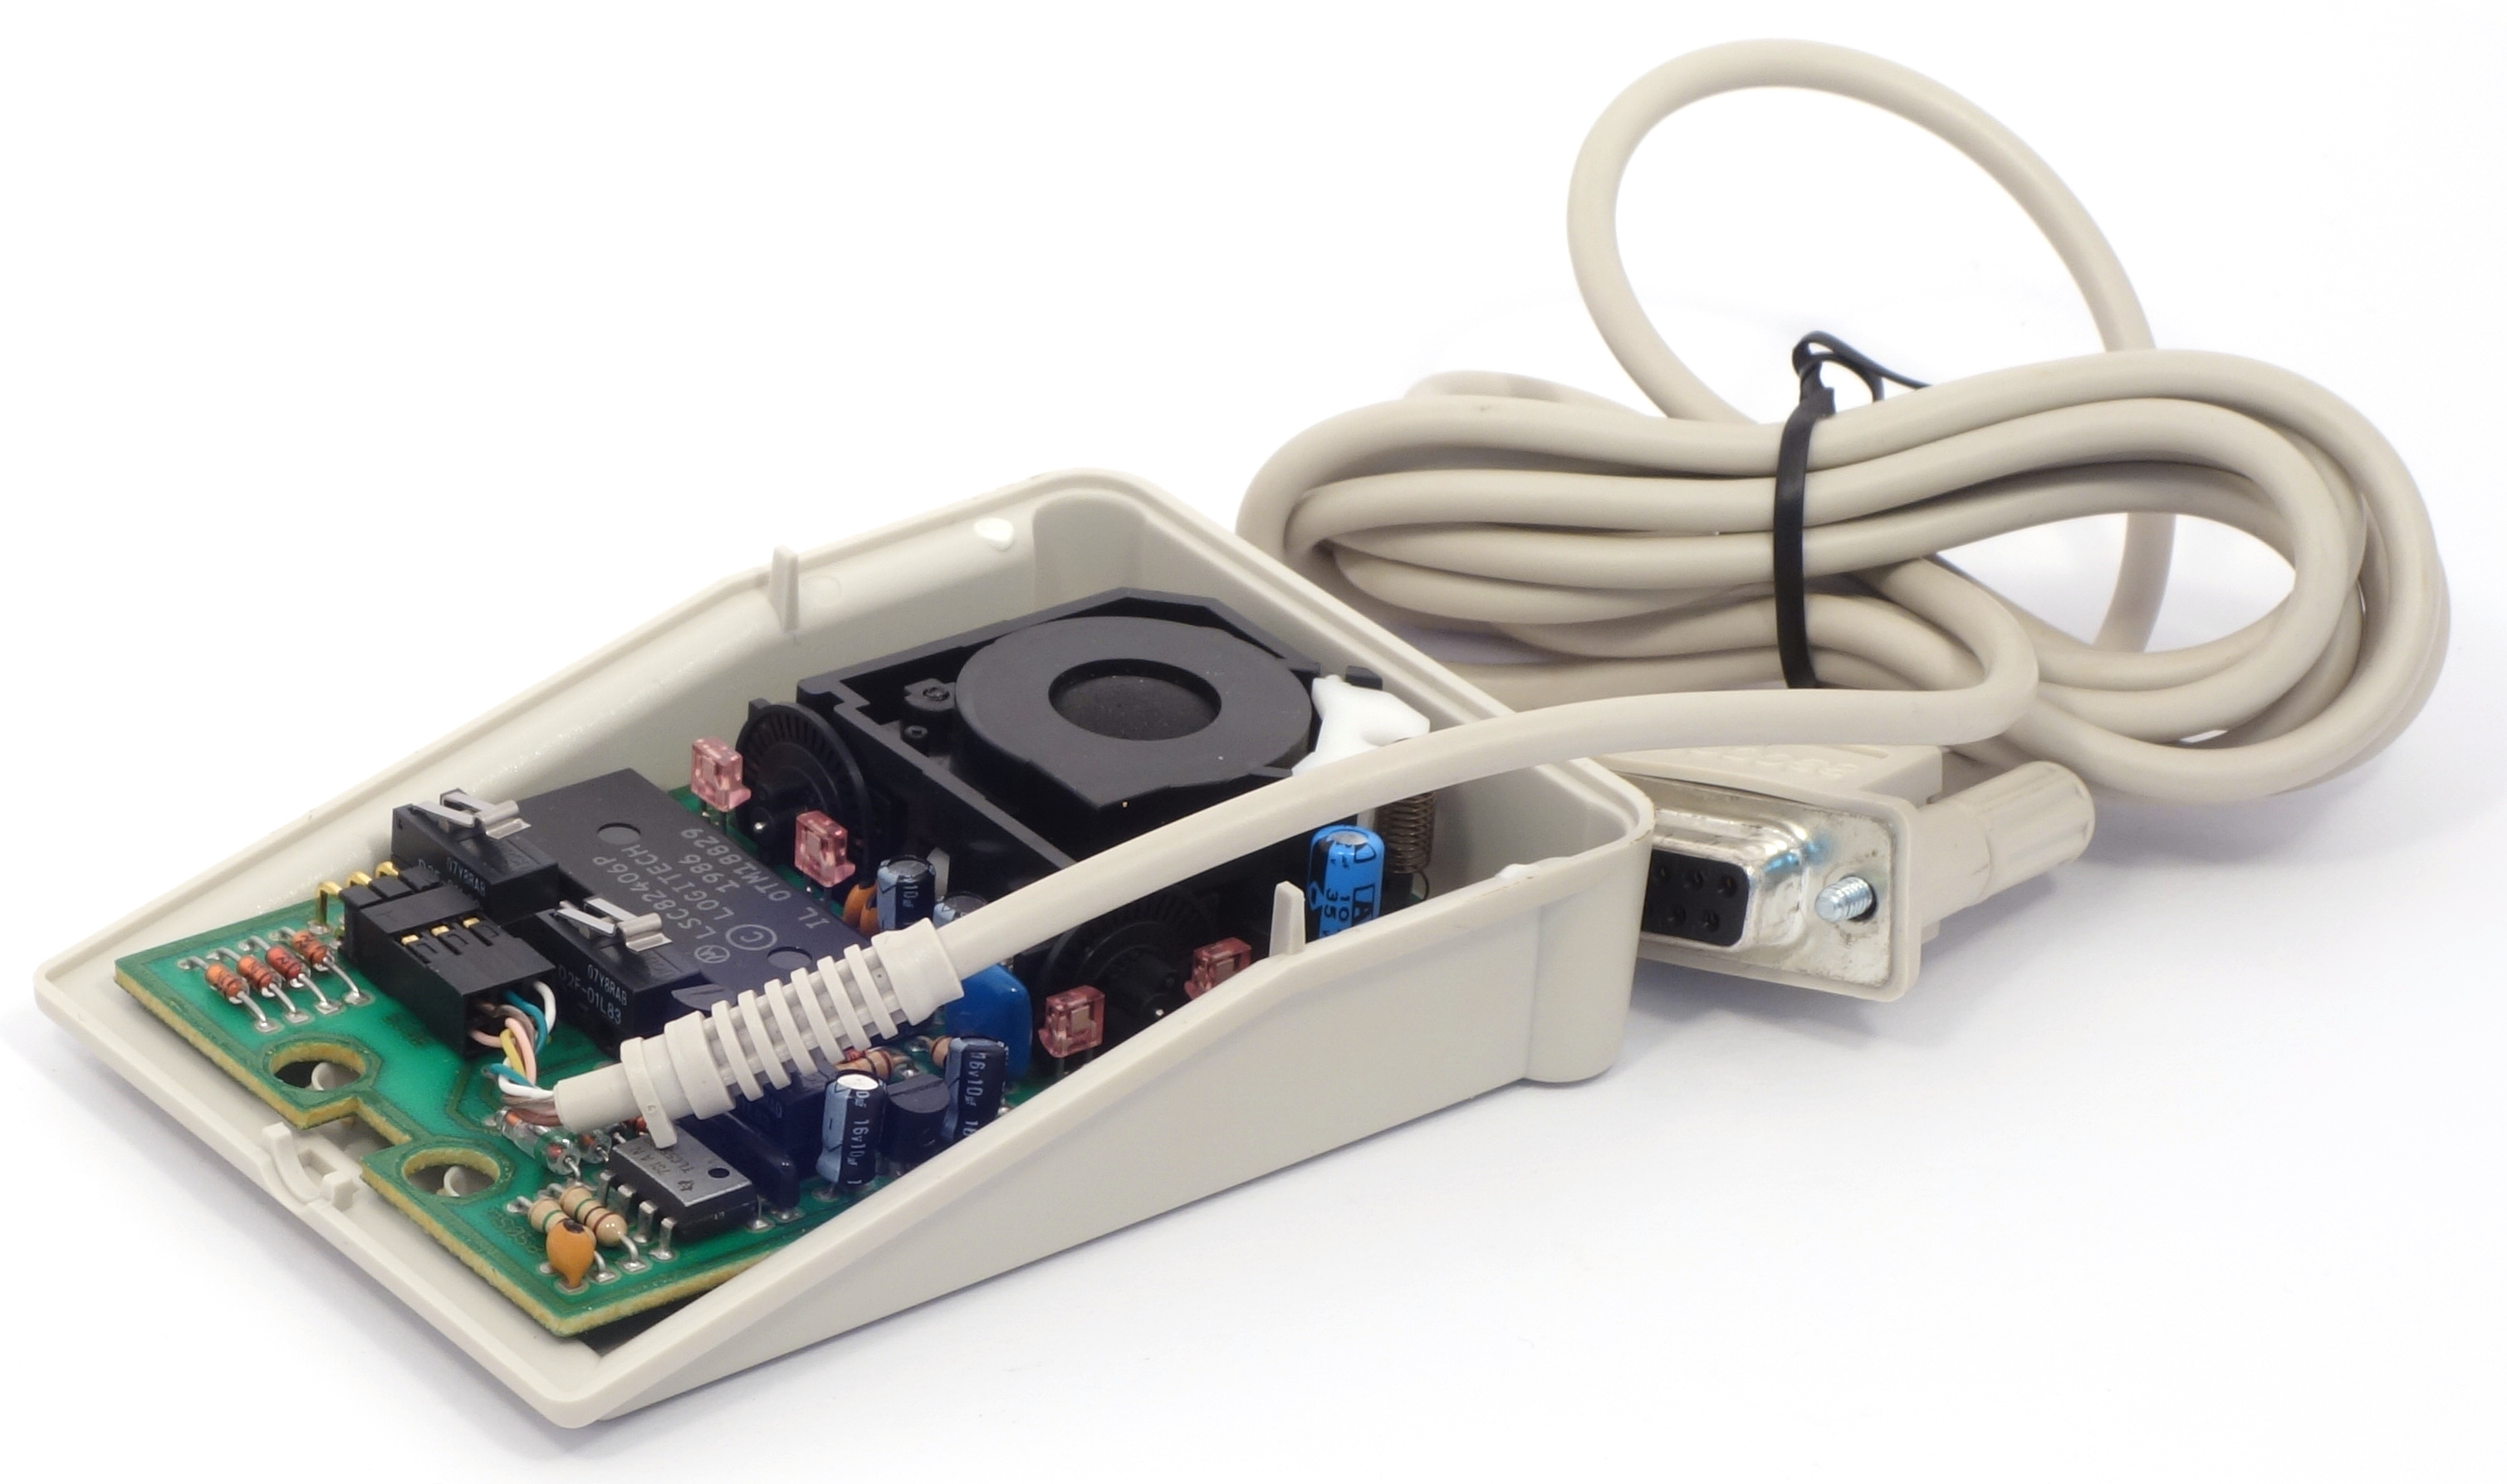
\includegraphics[scale=0.7]{1985_logitech_c7_mouse/inside_60.jpg}
    \caption{Logitech C7 mouse disassembled}
    \label{fig:LogitechC7Inside}
\end{figure}

\begin{thebibliography}{9}
\bibitem {history} Logitech History. 2007 \url{https://web.archive.org/web/20081221120203/http://www.logitech.com/lang/pdf/logitech_history_200703.pdf}
\bibitem {timeline} Mouse timeline scroll by Logitech. Historic Firsts: The Mouse. Doug Engelbart Institute. \url{https://www.dougengelbart.org/content/view/162/#img1}
\bibitem {manual1} LOGIMOUSE C7 Technical Reference Manual. Firmware Revision 3.0. 1986. \url{https://bitsavers.org/pdf/logitech/mouse/Logitech_Logimouse_C7_Firmware_Rev_3.0_Jan86.pdf}
\bibitem {manual2} LOGITECH MOUSE User's Manual. Serial Mouse, Bus Mouse, Series 2 Mouse. 1987. \url{https://bitsavers.org/pdf/logitech/mouse/Logitech_Mouse_Users_Manual_Feb87.pdf}
\end{thebibliography}
\end{document}
